\section{Рабочий проект}

\subsection{Спецификация компонентов и классов программы}

\subsubsection{Модули программной системы}

\paragraph{Модуль main.py}

Модуль предоставляет графический интерфейс с меню для переключения между тремя режимами работы: анализ изображений, обучение и тестирование нейронной сети. 

Класс -- MainWindow.

Описание класса MainWindow:
Класс предназначен для управления главным окном приложения и переключения между режимами работы программы. Базовый класс -- QMainWindow, стандартный класс библиотеки PyQt5. Интерфейсы: панель меню, позволяющая переключать режимы работы программы; центральный виджет QStackedWidget, отображающий интерфейс активного режима работы. Константы: отсутствуют. Внутренние поля:
\begin{itemize}
	\item stack: QStackedWidget -- содержит три виджета графического интерфейса для каждого режима работы программы;
	\item analysis\_widget: ImageAnalysisWidget -- виджет, содержащий графический интерфейс режима анализа изображений;
	\item training\_widget: TrainingWidget -- виджет, содержащий графический интерфейс режима обучения нейронной сети;
	\item testing\_widget: TestingWidget -- виджет, содержащий графический интерфейс режима тестирования нейронной сети.
\end{itemize}
Методы класса представлены в таблице~\ref{table:main_method}.
\renewcommand{\arraystretch}{0.8} % уменьшение расстояний до сетки таблицы
\begin{xltabular}{\textwidth}{|X|>{\setlength{\baselineskip}{0.7\baselineskip}}p{4cm}|p{6cm}|}
	\caption{Методы класса MainWindow\label{table:main_method}}\\
	\hline 
	\centrow \setlength{\baselineskip}{0.7\baselineskip} Название метода & 
	\centrow Область видимости & 
	\centrow Назначение метода \\ 
	\hline 
	\endfirsthead
	
	\caption*{Продолжение таблицы \ref{table:main_method}}\\
	\hline 
	\centrow Название метода & 
	\centrow Область видимости &
	\centrow Назначение метода \\ 
	\hline 
	\endhead
	
	\_\_init\_\_ & Внутренний  & Инициализирует главное окно программы, задает его параметры, заголовок, панель меню с действиями для переключения режимов \\ \hline 
	switch\_mode & Общедоступный & Переключает графический интерфейс в соответствии с выбранным режимом работы \\ \hline
	
\end{xltabular}
\renewcommand{\arraystretch}{1.0} % восстановление сетки
\vspace{-\baselineskip}
Метод \_\_init\_\_ не имеет входных и возвращаемых данных. 
Метод switch\_mode. Входные данные: index (тип int) -- идентификатор виджета активного режима окна. Возвращаемых данных нет.

\paragraph{Модуль model.py}

Модуль определяет структуру нейронной сети UNet, используемой для обнаружения разливов нефти.

Класс -- UNet.

Описание класса UNet:
Класс реализует модель UNet для сегментации и распознавания пятен нефтяных разливов на поверхности водоемов. Базовый класс --  nn.Module, стандартный класс библиотеки PyTorch. Интерфейсы: общедоступные методы \_\_init\_\_ и forward. Константы отсутствуют. Внутренние поля:
\begin{itemize}
	\item enc1: nn.Sequential -- первый блок энкодера;
	\item enc2: nn.Sequential -- второй блок энкодера;
	\item pool: nn.MaxPool2d -- слой максимального пуллинга, уменьшающий разрешение;
	\item bottleneck: nn.Sequential -- блок узкого места;
	\item upconv2: nn.ConvTranspose2d -- второй слой повышения разрешения;
	\item dec2: nn.Sequential -- второй блок декодера;
	\item upconv1: nn.ConvTranspose2d -- первый слой повышения разрешения;
	\item dec1: nn.Sequential -- первый блок декодера;
	\item final\_conv: nn.Conv2d -- финальный сверточный слой, создающий выходную маску признаков.
\end{itemize}
Методы класса представлены в таблице~\ref{table:model_method}
\renewcommand{\arraystretch}{0.8} % уменьшение расстояний до сетки таблицы
\begin{xltabular}{\textwidth}{|X|>{\setlength{\baselineskip}{0.7\baselineskip}}p{4cm}|p{6cm}|}
	\caption{Методы класса UNet\label{table:model_method}}\\
	\hline 
	\centrow \setlength{\baselineskip}{0.7\baselineskip} Название метода & 
	\centrow Область видимости & 
	\centrow Назначение метода \\ 
	\hline 
	\endfirsthead
	
	\caption*{Продолжение таблицы \ref{table:model_method}}\\
	\hline 
	\centrow Название метода & 
	\centrow Область видимости &
	\centrow Назначение метода \\ 
	\hline 
	\endhead
	
	\_\_init\_\_ & Общедоступный  & Инициализирует архитектуру UNet \\ \hline 
	forward & Общедоступный & Выполняет прямой проход через нейронную сеть, возвращая итог сегментации \\ \hline
	conv\_block & Внутренний & Определяет сверточный блок с двумя сверточными слоями и функциями активации\\ \hline
	
\end{xltabular}
\renewcommand{\arraystretch}{1.0} % восстановление сетки
\vspace{-\baselineskip}
Метод  \_\_init\_\_. Входные данные: 
\begin{itemize}
	\item in\_channels (тип int, значение по умолчанию -- 1) -- количество входных каналов;
	\item out\_channels (тип int, значение по умолчанию -- 1) -- количество выходных каналов.
\end{itemize}
Возвращаемых данных нет.

Метод forward. Входные данные: x (объект torch.Tensor формы (batch\_size, in\_channels, height, width)) -- входной тензор. Возвращаемые данные: объект torch.Tensor -- выходная маска признаков сходной формы.

Метод conv\_block. Входные данные:
\begin{itemize}
	\item in\_c (тип int) -- входные каналы.
	\item out\_c (тип int) -- выходные каналы. 
\end{itemize}
Возвращаемые данные: объект nn.Sequential -- контейнер сверточного блока.

\paragraph{Модуль test.py}

Модуль содержит функции для оценки обученной модели UNet на одном изображении.  Не содержит классов. Методы модуля:
\begin{enumerate}
	\item dice\_coefficient. Вычисляет коэффициент Dice для предсказанной маски. Входные данные:
	\begin{itemize}
		\item pred (тип torch.Tensor) -- предсказанная маска;
		\item target (тип torch.Tensor ) -- целевая маска;
		\item smooth (тип float,  значение по умолчанию -- 1e$^{-6} $) -- стабилизирующая константа для избежания деления на ноль.
	\end{itemize}
	Возвращаемые данные -- коэффициент Dice в виде float-числа.
	\item iou\_score. Вычисляет пересечение по объединению (коэффициент IoU) для предсказанной маски. Входные данные:
	\begin{itemize}
		\item pred (тип torch.Tensor) -- предсказанная маска;
		\item target (тип torch.Tensor ) -- целевая маска;
		\item smooth (тип float,  значение по умолчанию -- 1e$^{-6} $) -- стабилизирующая константа для избежания деления на ноль.
	\end{itemize}
	Возвращаемые данные -- коэффициент пересечения по объединению в виде float-числа.
	\item load\_image. Загружает изображение и выполняет предобработку для дальнейшего анализа нейронной сетью. Входные данные:
	\begin{itemize}
		\item path (тип str) -- путь к загружаемому изображению;
		\item size (тип tuple) -- целевой размер изображения для дальнейшей обработки нейронной сетью.
	\end{itemize}
	Возвращаемые данные: нормализованный массив изображения типа np.ndarray.
	\item run\_evaluation. Выполняет оценку точности обученной модели нейронной сети и возвращает результаты обработки и метрики. Входные данные:
	\begin{itemize}
		\item image\_path (тип str) -- путь к анализируемому изображению;
		\item weights (тип str) -- путь к оцениваемым весам модели;
		\item threshold (тип float, значение по умолчанию = 0,5) -- порог для бинаризации масок
	\end{itemize}
	Возвращаемые данные -- значения коэффициентов Dice и IoU, исходное изображение, ожидаемую маску, полученную при помощи пороговой бинаризации и предсказанную сетью маску в виде словаря dict.
\end{enumerate}

\paragraph{Модуль train.py}

Модуль управляет загрузкой датасета и обучением нейронной сети.

Классы: dataset и Trainer.

Описание класса dataset:
Класс загружает и предобрабатывает изображения и создает псевдомаски на основании порога для обучения нейронной сети. Базовый класс -- Dataset, стандартный класс библиотеки PyTorch. Интерфейсы -- общедоступные методы \_\_init\_\_, \_\_len\_\_, \_\_getitem\_\_, общедоступные атрибуты image\_dir, images. Константы отсутствуют. Внутренние поля: 
\begin{itemize}
	\item image\_dir: str -- папка, содержащая датасет;
	\item images: list -- список имен файлов изображений для обучения;
	\item threshold: float -- порог для создания обучающих масок.
\end{itemize}
Методы класса представлены в таблице~\ref{table:dataset_method}. 
\renewcommand{\arraystretch}{0.8} % уменьшение расстояний до сетки таблицы
\begin{xltabular}{\textwidth}{|X|>{\setlength{\baselineskip}{0.7\baselineskip}}p{4cm}|p{6cm}|}
	\caption{Методы класса dataset\label{table:dataset_method}}\\
	\hline 
	\centrow \setlength{\baselineskip}{0.7\baselineskip} Название метода & 
	\centrow Область видимости & 
	\centrow Назначение метода \\ 
	\hline 
	\endfirsthead
	
	\caption*{Продолжение таблицы \ref{table:dataset_method}}\\
	\hline 
	\centrow Название метода & 
	\centrow Область видимости &
	\centrow Назначение метода \\ 
	\hline 
	\endhead
	
	\_\_init\_\_ & Общедоступный  & Инициализирует датасет, проверяя директорию и загружая имена файлов изображений \\ \hline 
	\_\_len\_\_ & Общедоступный & Определяет количество изображений в датасете \\ \hline
	\_\_getitem\_\_ & Общедоступный & Загружает, предобрабатывает и создает обучающую маску для изображений датасета \\ \hline
	
\end{xltabular}
\renewcommand{\arraystretch}{1.0} % восстановление сетки
\vspace{-\baselineskip}
Метод \_\_init\_\_. Входные данные:
\begin{itemize}
	\item image\_dir (тип str) -- путь к папке с датасетом;
	\item threshold (тип float, значение по умолчанию -- 0,5) -- порог для создания обучающих масок.
\end{itemize}

Метод \_\_len\_\_. Входные данные отсутствуют. Возвращаемые данные -- количество изображений в датасете в виде int-числа.

Метод \_\_getitem\_\_. Входные данные: idx (тип int) -- порядковый номер обрабатываемого изображения. Возвращаемые данные -- тензор изображения и маски в виде кортежа tuple[torch.Tensor, torch.Tensor].

Описание класса Trainer:
Класс управляет обучением модели нейронной сети и отправляет сигналы о состоянии процесса обучения для обновления графического интерфейса. Базовый класс -- QObject, стандартный класс библиотеки PyQt5. Интерфейсы -- сигналы о состоянии процесса обучения, общедоступный метод \_\_init\_\_. Константы отсутствуют. Внутренние поля: 
\begin{itemize}
	\item epoch\_start\_signal: pyqtSignal[int, int] -- сигнал начала эпохи, содержащий её номер и общее количесвто эпох;
	\item epoch\_complete\_signal: pyqtSignal[int, float] -- сигнал завершения эпохи, содержащий её номер и среднее значение потери при обучении;
	\item batch\_progress\_signal: pyqtSignal[int, int, float] -- сигнал прогресса обработки батча, содержащий его номер, потерю, общее число батчей;
	\item training\_complete\_signal: pyqtSignal[str] -- сигнал завершения обучения.
\end{itemize}
Методы класса представлены в таблице~\ref{table:Trainer_method}
\renewcommand{\arraystretch}{0.8} % уменьшение расстояний до сетки таблицы
\begin{xltabular}{\textwidth}{|X|>{\setlength{\baselineskip}{0.7\baselineskip}}p{4cm}|p{6cm}|}
	\caption{Методы класса Trainer\label{table:Trainer_method}}\\
	\hline 
	\centrow \setlength{\baselineskip}{0.7\baselineskip} Название метода & 
	\centrow Область видимости & 
	\centrow Назначение метода \\ 
	\hline 
	\endfirsthead
	
	\caption*{Продолжение таблицы \ref{table:Trainer_method}}\\
	\hline 
	\centrow Название метода & 
	\centrow Область видимости &
	\centrow Назначение метода \\ 
	\hline 
	\endhead
	
	\_\_init\_\_ & Общедоступный  & Инициализирует процесс обучения с определенными параметрами \\ \hline 
	run & Общедоступный & Обучает нейронную сеть, отправляя сигналы о прогрессе, и сохраняет параметры модели по завершении обучения \\ \hline
	
\end{xltabular}
\renewcommand{\arraystretch}{1.0} % восстановление сетки
\vspace{-\baselineskip}

Метод \_\_init\_\_. Входные данные:
\begin{itemize}
	\item image\_dir (тип str) -- путь датасета;
	\item save\_path (тип str) -- путь сохранения параметров обученной модели;
	\item batch\_size (тип int, значение по умолчанию -- 1) -- размер батча;
	\item epochs (тип int, значение по умолчанию -- 25) -- количество обучающих эпох;
	\item lr (тип float, значение по умолчанию --  1e$^{-4} $) -- скорость обучения;
	\item threshold (тип float, значение по умолчанию -- 0,5) -- порог для обучающих масок.
\end{itemize}
Возвращаемых данных нет. 

Функция run не имеет входных и возвращаемых данных.

В модуле train.py также реализован метод main(), предназначенная для получения аргументов обучения из графического интерфейса и запуска обучения при помощи Trainer. Метод не имеет входных и возвращаемых данных.

\paragraph{Модуль detect.py}

Модуль используется для анализа изображений с использованием обученной модели нейронной сети, обнаруживая и выделяя пятна нефтяных разливов.  Не содержит классов. Методы модуля:
\begin{enumerate}
	\item load\_model. Загружает и инициализирует модель нейронной сети с указанными параметрами. Входные данные -- model\_path (тип str) -- путь к файлу параметров модели. Возвращаемые данные -- элемент класса Unet модуля model.py с загруженными из файла весами.
	\item analyze\_return. Метод обрабатывает изображение, используя нейронную сеть, создает бинарную маску разлива и возвращает исходное изображение с выделенными распознанными пятнами нефтяных разливов. Входные данные:
	\begin{itemize}
		\item image\_path (тип str) -- путь к анализируемому изображению;
		\item model\_path (тип str) -- путь к файлу параметров нейронной сети;
		\item threshold (тип float, значение по умолчанию -- 0,5) -- порог для бинаризации маски.
	\end{itemize}
	Возвращаемые данные -- изображение с выделенными распознанными нефтяными пятнами в формате np.ndarray.
\end{enumerate}

\paragraph{Модуль analyze\_ui.py}

Модуль содержит графический интерфейс режима анализа изображений с использованием предварительно обученной модели нейронной сети.

Класс -- ImageAnalysisWidget. 

Описание класса ImageAnalysisWidget:
Класс содержит графический интерфейс, позволяющий выбрать анализируемое изображение, файл параметров нейронной сети, запустить процесс анализа и сохранить результат и отображающий этот результат. Базовый класс -- QWidget, стандартный класс библиотеки PyQt5. Интерфейсы -- поля для путей к изображению и модели, кнопки для выбора этих путей, начала анализа, сохранения результата, область отображения изображения. Константы отсутствуют. Внутренние поля класса:
\begin{itemize}
	\item image\_path: str -- путь к выбранному изображению;
	\item model\_path: str -- путь к выбранному файлу параметров нейронной сети;
	\item result\_img: np.ndarray -- проанализированное изображение с разметкой;
	\item path\_label: QLabel -- надпись "<Изображение для анализа:">;
	\item path\_field: QTextEdit -- текстовое поле для отображения пути к выбранному изображению;
	\item select\_button: QPushButton -- кнопка для выбора изображения;
	\item model\_label: QLabel -- надпись "<Путь к модели нейросети:">;
	\item model\_path\_field: QTextEdit -- текстовое поле для отображения пути к выбранному файлу параметров нейронной сети;
	\item select\_model\_button: QPushButton -- кнопка для выбора файла параметров нейронной сети;
	\item image\_label: QLabel -- поле для отображения входного или проанализированного изображения;
	\item analyze\_button: QPushButton -- кнопка для анализа изображения;
	\item save\_button: QPushButton -- кнопка для сохранения результата анализа.
\end{itemize}
Методы класса представлены в таблице~\ref{table:analyze_ui_method}
\renewcommand{\arraystretch}{0.8} % уменьшение расстояний до сетки таблицы
\begin{xltabular}{\textwidth}{|X|>{\setlength{\baselineskip}{0.7\baselineskip}}p{4cm}|p{6cm}|}
	\caption{Методы класса ImageAnalysisWidget\label{table:analyze_ui_method}}\\
	\hline 
	\centrow \setlength{\baselineskip}{0.7\baselineskip} Название метода & 
	\centrow Область видимости & 
	\centrow Назначение метода \\ 
	\hline 
	\endfirsthead
	
	\caption*{Продолжение таблицы \ref{table:analyze_ui_method}}\\
	\hline 
	\centrow Название метода & 
	\centrow Область видимости &
	\centrow Назначение метода \\ 
	\hline 
	\endhead
	
	\_\_init\_\_ & Общедоступный  & Инициализирует графический интерфейс, включая его макет и элементы  \\ \hline 
	select\_image & Общедоступный & Открывает диалоговое окно выбора изображения, отображает путь к нему и само изображение в интерфейсе \\ \hline
	select\_model & Общедоступный & Открывает диалоговое окно выбора файла настроек модели и отображает путь к нему \\ \hline
	analyze\_image & Общедоступный & Анализирует загруженное изображение при помощи нейронной сети и отображает результат распознавания \\ \hline
	save\_result & Общедоступный & Открывает диалоговое окно выбора папки сохранения результата анализа изображения и сохраняет результат \\ \hline
	
\end{xltabular}
\renewcommand{\arraystretch}{1.0} % восстановление сетки
\vspace{-\baselineskip}
Методы в этом классе не имеют входных и возвращаемых данных.

\paragraph{Модуль train\_ui.py}

Модуль содержит графический интерфейс для настройки параметров и запуска процесса обучения модели нейронной сети.

Классы: TrainingThread, TrainingWidget.

Описание класса TrainingThread:
Данный класс выполняет процесс обучений нейронной сети в отдельном потоке для избежания блокировки и зависания графического интерфейса. Базовый класс -- QThread, стандартный класс библиотеки PyQt5. Интерфейсы -- сигналы для передачи прогресса обучения и обработки ошибок, функция, управляющая процессом обучения. Константы отсутствуют. Внутренние поля:
\begin{itemize}
	\item trainer: Trainer -- экземпляр класса Trainer из train.py для обучения нейронной сети;
	\item error\_signal: pyqtSignal[str] -- сигнал для передачи сообщений об ошибках.
\end{itemize}
Методы класса представлены в таблице~\ref{table:TrainingThread_method}
\renewcommand{\arraystretch}{0.8} % уменьшение расстояний до сетки таблицы
\begin{xltabular}{\textwidth}{|X|>{\setlength{\baselineskip}{0.7\baselineskip}}p{4cm}|p{6cm}|}
	\caption{Методы класса TrainigThread\label{table:TrainingThread_method}}\\
	\hline 
	\centrow \setlength{\baselineskip}{0.7\baselineskip} Название метода & 
	\centrow Область видимости & 
	\centrow Назначение метода \\ 
	\hline 
	\endfirsthead
	
	\caption*{Продолжение таблицы \ref{table:TrainingThread_method}}\\
	\hline 
	\centrow Название метода & 
	\centrow Область видимости &
	\centrow Назначение метода \\ 
	\hline 
	\endhead
	
	\_\_init\_\_ & Общедоступный  & Инициализирует поток обучения нейронной сети с экземпляром класса Trainer  \\ \hline 
	run & Общедоступный & Выполняет обучение нейронной сети с обработкой ошибок \\ \hline
	
\end{xltabular}
\renewcommand{\arraystretch}{1.0} % восстановление сетки
\vspace{-\baselineskip}
Метод \_\_init\_\_. Входные данные:
\begin{itemize}
	\item dataset\_path (тип str) -- путь к датасету;
	\item model\_path (тип str) -- путь к директории сохранения модели;
	\item batch\_size (тип int) -- размер батча;
	\item epochs (тип int) -- количество эпох обучения.
\end{itemize}
Возвращаемых данных нет.

Метод run не имеет входных и возвращаемых данных.

Описание класса TrainingWidget:
Класс предоставляет графиеский интерфейс для выбора параметров обучения и отображения прогресса. Базовый класс -- QWidget, стандартный класс PyQt5. Интерфейсы -- поля ввода расположений датасета и сохранения результата, кнопки выбора путей, запуска обучения, шкала прогресса завершения обучения, текстовое поле для отображения сведений об обучении. Константы отсутствуют. Внутренние поля:
\begin{itemize}
	\item dataset\_label: QLabel -- надпись "<Папка датасета:">;
	\item dataset\_path\_field: QTextEdit -- поле для отображения выбранной папки датасета;
	\item select\_dataset\_button: QPushButton -- кнопка для выбора папки датасета;
	\item model\_label: QLabel -- надпись "<Папка сохранения:">;
	\item model\_path\_field: QTextEdit -- поле для отображения выбранной папки сохранения;
	\item select\_model\_button: QPushButton -- кнопка для выбора папки сохранения;
	\item batch\_size\_label: QLabel -- надпись "<Размер батча:">;
	\item batch\_size\_combo: QComboBox -- выпадающий список для выбора размера батча;
	\item epochs\_label: QLabel -- надпись "<Количество эпох:">;
	\item epochs\_field: QLineEdit -- поле для ввода количества эаох обучения;
	\item progress\_label: QLabel -- надпись "<Прогресс эпохи:">;
	\item progress\_bar: QProgressBar -- шкала прогресса обучения нейронной сети;
	\item log\_label: QLabel -- надпись "<Процесс выполнения:">;
	\item output\_text: QTextEdit -- поле для отображения сведений о процессе обучения;
	\item train\_button: QPushButton -- кнопка для запуска обучения;
	\item thread: TrainingThread -- поток для процесса обучения.
\end{itemize}
Методы класса представлены в таблице~\ref{table:TrainingThread_method}.
\renewcommand{\arraystretch}{0.8} % уменьшение расстояний до сетки таблицы
\begin{xltabular}{\textwidth}{|X|>{\setlength{\baselineskip}{0.7\baselineskip}}p{4cm}|p{6cm}|}
	\caption{Методы класса TrainigWidget\label{table:TrainingWidget_method}}\\
	\hline 
	\centrow \setlength{\baselineskip}{0.7\baselineskip} Название метода & 
	\centrow Область видимости & 
	\centrow Назначение метода \\ 
	\hline 
	\endfirsthead
	
	\caption*{Продолжение таблицы \ref{table:TrainingWidget_method}}\\
	\hline 
	\centrow Название метода & 
	\centrow Область видимости &
	\centrow Назначение метода \\ 
	\hline 
	\endhead
	
	\_\_init\_\_ & Общедоступный  & Инициализирует графический интерфейс, включая макет и элементы для настройки обучения и отображения прогресса  \\ \hline 
	select\_dataset\_folder & Общедоступный & Открывает диалоговое окно для выбора папки, содержащей датасет \\ \hline
	select\_model\_path & Общедоступный & Открывает диалоговое окно для выбора папки сохранения весов обученной нейронной сети \\ \hline
	run\_training & Общедоступный & Проверяет корректность параметров обучения, заданных пользователем, отображает ошибки при наличии, создает поток обучения, подключает сигналы для обновления графического интерфейса \\ \hline
	on\_epoch\_start & Общедоступный & Обновляет отображаемый журнал обучения нейронной сети записью о начале эпохи и сбрасывает шкалу прогресса при начале новой эпохи обучения \\ \hline
	on\_epoch\_complete & Общедоступный & Обновляет отображаемый журнал информацией о завершении эпохи и заполняет шкалу прогресса по окончании эпохи обучения\\ \hline
	on\_batch\_progress & Общедоступный & Обновляет шкалу прогресса в процессе обучения \\ \hline
	append\_output & Общедоступный & Добавляет текст в область отображения журнала \\ \hline
	show\_error & Общедоступный & Отображает диалоговое окно ошибки \\ \hline
	
\end{xltabular}
\renewcommand{\arraystretch}{1.0} % восстановление сетки
\vspace{-\baselineskip}
Методы \_\_init\_\_, select\_dataset\_folder, select\_model\_path, run\_training не имеют входных и возвращаемых данных.

Метод on\_epoch\_start. Входные данные:
\begin{itemize}
	\item epoch (тип int) -- номер текущей эпохи обучения;
	\item total\_epochs (тип int) -- общее количество эпох.
\end{itemize}
Возвращаемых данных нет.

Метод on\_epoch\_complete. Входные данные:
\begin{itemize}
	\item epoch (тип int) -- номер завершенной эпохи;
	\item avg\_loss (тип float) -- среднее значение потери за эпоху обучения.
\end{itemize}
Возвращаемых данных нет.

Метод on\_batch\_progress. Входные данные:
\begin{itemize}
	\item batch (тип int) -- номер текущего батча;
	\item total\_batches (тип int) -- общее количество батчей;
	\item loss (тип float) -- значение потери для текущего батча.
\end{itemize}
Возвращаемых данных нет.

Метод append\_output. Входные данные -- text (тип str) -- текст, добавляемый в журнал обучения. Возвращаемых данных нет.

Метод show\_error. Входные данные -- error\_message (тип str) -- отображаемое сообщение об ошибке. Возвращаемых данных нет.

\paragraph{Модуль test\_ui.py}

Модуль предоставляет графический интерфейс для тестирования модели нейронной сети.

Классы: TestingThread, TestingWidget.

Описание класса TestingThread:
Класс выполняет оценку модели в отдельном потоке, чтобы избежать зависаний графического интерфейса. Базовый класс -- QThread, стандартный класс PyQt5. Интерфейсы класса -- сигналы для обновления графического интерфейса. Константы отсутствуют. Внутренние поля:
\begin{itemize}
	\item image\_path: str -- путь к тестовому изображению;
	\item model\_path: str -- путь к файлу настроек модели нейронной сети;
	\item output\_signal: pyqtSignal[str] -- сигнал для сообщений о результатах тестирования;
	\item results\_signal: pyqtSignal[dict] -- сигнал для результатов оценки;
	\item error\_signal: pyqtSignal[str] -- сигнал для сообщений об ошибках.
\end{itemize}
Методы класса представлены в таблице~\ref{table:TestingThread_method}
\renewcommand{\arraystretch}{0.8} % уменьшение расстояний до сетки таблицы
\begin{xltabular}{\textwidth}{|X|>{\setlength{\baselineskip}{0.7\baselineskip}}p{4cm}|p{6cm}|}
	\caption{Методы класса TestingThread\label{table:TestingThread_method}}\\
	\hline 
	\centrow \setlength{\baselineskip}{0.7\baselineskip} Название метода & 
	\centrow Область видимости & 
	\centrow Назначение метода \\ 
	\hline 
	\endfirsthead
	
	\caption*{Продолжение таблицы \ref{table:TestingThread_method}}\\
	\hline 
	\centrow Название метода & 
	\centrow Область видимости &
	\centrow Назначение метода \\ 
	\hline 
	\endhead
	
	\_\_init\_\_ & Общедоступный  & Инициализирует поток, передавая в него пути к тестовому изображению и папке модели  \\ \hline 
	run & Общедоступный & Выполняет оценку нейронной сети, отправляя результаты или ошибки через сигналы  \\ \hline
	
\end{xltabular}
\renewcommand{\arraystretch}{1.0} % восстановление сетки
\vspace{-\baselineskip}
Метод \_\_init\_\_. Входные данные:
\begin{itemize}
	\item image\_path (тип str) -- путь к тестовому изображению;
	\item model\_path (тип str) -- путь к файлу параметров нейронной сети.
\end{itemize}
Возвращаемых данных нет.

Метод run не имеет входных и возвращаемых данных.

Описание класса TestingWidget:
Класс содержит графический интерфейс для выбора тестового изображения и файла весов модели, запуска оценки и отображения полученных метрик точности нейронной сети, целевой и предсказанной масок. Базовый класс -- QWidget, стандартный класс PyQt5. Интерфейсы класса -- поля для отображения путей к тестовому изображению и файлу весов, кнопки для выбора этих файлов и запуска тестирования, области для отображения изображений и метрик. Константы отсутствуют. Внутренние поля:
\begin{itemize}
	\item image\_path: str -- путь к тестовому изображению;
	\item model\_path: str -- путь к тестируемым параметрам модели;
	\item path\_label: QLabel -- надпись "<Изображение для проверки модели:">;
	\item image\_path\_field: QTextEdit -- поле для отображения пути к выбранному изображению;
	\item select\_image\_button: QPushButton -- кнопка для выбора изображения;
	\item model\_label: QLabel -- надпись "<Путь к параметрам нейросети:">;
	\item model\_path\_field: QTextEdit -- поле для отображения пути к выбранному файлу параметров нейронной сети;
	\item select\_model\_button: QPushButton -- кнопка для выбора модели;
	\item output\_text: QTextEdit -- поле для отображения метрик точности нейронной сети;
	\item input\_text\_label: QLabel -- надпись "<Исходное изображение">;
	\item input\_image\_label: QLabel -- поле для отображения изображения;
	\item gt\_text\_label: QLabel -- надпись "<Ожидаемый результат">;
	\item gt\_mask\_label: QLabel -- поле для отображения целевой маски;
	\item pred\_text\_label: QLabel -- надпись "<Результат работы модели">;
	\item pred\_mask\_label: QLabel -- поле для отображения предсказанной маски;
	\item test\_button: QPushButton -- кнопка для запуска тестирования;
	\item thread: TestingThread -- поток для выполнения тестирования и оценки.
\end{itemize}
Методы класса представлены в таблице~\ref{table:TestingWidget_method}
\renewcommand{\arraystretch}{0.8} % уменьшение расстояний до сетки таблицы
\begin{xltabular}{\textwidth}{|X|>{\setlength{\baselineskip}{0.7\baselineskip}}p{4cm}|p{6cm}|}
	\caption{Методы класса TestingWidget\label{table:TestingWidget_method}}\\
	\hline 
	\centrow \setlength{\baselineskip}{0.7\baselineskip} Название метода & 
	\centrow Область видимости & 
	\centrow Назначение метода \\ 
	\hline 
	\endfirsthead
	
	\caption*{Продолжение таблицы \ref{table:TestingWidget_method}}\\
	\hline 
	\centrow Название метода & 
	\centrow Область видимости &
	\centrow Назначение метода \\ 
	\hline 
	\endhead
	
	\_\_init\_\_ & Общедоступный  & Инициализирует графический интерфейс, включая макет и элементы для тестирования и отображения результатов  \\ \hline 
	select\_image & Общедоступный & Открывает диалоговое окно для выбора тестового изображения и добавляет путь в специальное поле \\ \hline
	select\_model & Общедоступный & Открывает диалоговое окно для выбора файла весов нейронной сети и добавляет путь в специальное поле \\ \hline
	run\_testing & Общедоступный & Проверяет входные данные, запускает поток тестирования и подключает сигналы для отображения результатов и ошибок \\ \hline
	show\_results& Общедоступный & Отображает исходное изображения и результаты тестирования в графическом интерфейсе \\ \hline
	append\_output & Общедоступный & Добавляет текст в область отображения результатов тестирования \\ \hline
	show\_error & Общедоступный & Отображает диалоговое окно ошибки \\ \hline
	numpy\_to\_qimage & Внутренний & Преобразует маски результатов из массивов в изображения\\ \hline
	
\end{xltabular}
\renewcommand{\arraystretch}{1.0} % восстановление сетки
\vspace{-\baselineskip}
Методы \_\_init\_\_, select\_image, select\_model, run\_testing не имеют входных и возвращаемых значений. 

Метод show\_results. Входное значение -- results (тип dict) -- словарь с результатами тестирования нейронной сети. Возвращаемых данных не имеет.

Метод append\_output. Вохдное значение -- text (тип str) -- текст, отображаемый в области результатов тестирования. Возвращаемых данных не имеет.

Метод show\_error. Входное значение -- error\_message (тип str) -- отображаемое сообщение об ошибке. Возвращаемых данных не имеет.

Метод numpy\_to\_qimage. Входные значения:
\begin{itemize}
	\item np\_array (тип np.ndarray) -- массив, представляющий изображение;
	\item is\_grayscale (тип bool, значение по умолчанию -- True) -- флаг, определяющий, является ли изображение полутоновым.
\end{itemize}
Возвращаемое значение -- преобразованное изображение в формате QImage.

\subsection{Модульное тестирование разработанной программной системы}

Модульный тест для класса UNet из модуля model.py представлен на рисунке~\ref{model_test:image}.

\begin{figure}[H]
\begin{lstlisting}[language=Python]
import unittest
import torch
from model import UNet

class TestUNet(unittest.TestCase):
	def test_model_initialization(self):
		model = UNet(in_channels=1, out_channels=1)
		self.assertIsInstance(model, UNet, "Должен создаваться экземпляр UNet")
	
	def test_forward_pass(self):
		model = UNet(in_channels=1, out_channels=1)
		input_tensor = torch.randn(1, 1, 320, 624)
		output = model(input_tensor)
		self.assertEqual(output.shape, (1, 1, 320, 624), "Некорректный размер вывода")
		self.assertTrue(torch.all(output >= 0), "Выход должен быть ≥ 0")
		self.assertTrue(torch.all(output <= 1), "Выход должен быть ≤ 1")
\end{lstlisting}  
\caption{Модульный тест класса UNet}
\label{model_test:image}
\end{figure}

Результат тестирования:
\begin{figure}[H]
	\centering
	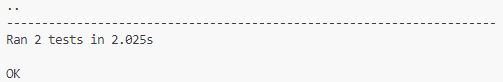
\includegraphics[width=0.7\linewidth]{images/model_test_results}
	\caption{Результат тестирования класса UNet}
	\label{fig:modeltestresults}
\end{figure}

Модульный тест для вычисления метрик модуля test.py представлен на рисунке~\ref{test_test:image}.

\begin{figure}[H]
	\begin{lstlisting}[language=Python]
import unittest
import torch
from test import dice_coefficient, iou_score

class TestMetrics(unittest.TestCase):
	def test_dice_coefficient(self):
		pred = torch.tensor([1, 1, 0, 0], dtype=torch.float32)
		target = torch.tensor([1, 0, 1, 0], dtype=torch.float32)
		dice = dice_coefficient(pred, target)
		self.assertTrue(0 <= dice <= 1, "Dice должен быть в [0, 1]")

	def test_iou_score(self):
		pred = torch.tensor([1, 1, 0, 0], dtype=torch.float32)
		target = torch.tensor([1, 0, 1, 0], dtype=torch.float32)
		iou = iou_score(pred, target)
		self.assertTrue(0 <= iou <= 1, "IoU должен быть в [0, 1]")
	\end{lstlisting}  
	\caption{Модульный тест функций подсчета метрик модуля test.py}
	\label{test_test:image}
\end{figure}

Результат тестирования:
\begin{figure}[H]
	\centering
	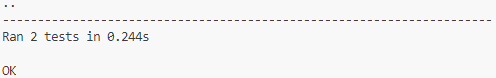
\includegraphics[width=0.7\linewidth]{images/test_test_results}
	\caption{Результат тестирования функций подсчета метрик модуля test.py}
	\label{fig:testtestresults}
\end{figure}

Модульный тест для класса analyze\_return из модуля detect.py представлен на рисунке~\ref{detect_test:image}.

\begin{figure}[H]
	\begin{lstlisting}[language=Python]
import unittest
import numpy as np
import cv2
import os
import torch
from unittest.mock import patch
from detect import analyze_return

	class TestDetect(unittest.TestCase):
		def setUp(self):
			self.test_img = np.random.randint(0, 255, (100, 100, 3), dtype=np.uint8)
			self.img_path = "test_image.jpg"
			cv2.imwrite(self.img_path, self.test_img)

		def tearDown(self):
			if os.path.exists(self.img_path):
			os.remove(self.img_path)

		@patch("detect.load_model")
		def test_analyze_save(self, mock_load_model):
			mock_model = mock_load_model.return_value
			mock_model.return_value = torch.sigmoid(torch.randn(1, 1, 320, 624))


			result = analyze_return(self.img_path, "dummy_model.pth")
			self.assertIsInstance(result, np.ndarray, "Должен возвращаться numpy-массив")
			self.assertEqual(result.shape[2], 3, "Изображение должно быть 3-канальным (BGR)")

	\end{lstlisting}  
	\caption{Модульный тест класса analyze\_return}
	\label{detect_test:image}
\end{figure}

Результат тестирования:
\begin{figure}[H]
	\centering
	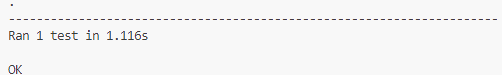
\includegraphics[width=0.7\linewidth]{images/detect_test_results}
	\caption{Результат тестирования класса analyze\_return}
	\label{fig:detecttestresults}
\end{figure}



\subsection{Системное тестирование разработанной программной системы}

Для проведения системного тестирования был использован файл весов, полученный после обучения нейронной сети на датасете, состоящем из 777 изображений. Обучение проводилось на протяжении после 25 эпох.

На рисунке~\ref{fig:ui_analysis_mode} представлено окно режима работы "<Анализ изображения">.
\begin{figure}[H]
	\centering
	\includegraphics[width=0.7\linewidth]{"images/анализ окно"}
	\caption{Окно программы в режиме "<Анализ изображения">}
	\label{fig:ui_analysis_mode}
\end{figure}

На рисунке~\ref{fig:analyze_select_image} представлено диалоговое окно выбора анализируемого изображения.

\begin{figure}[H]
	\centering
	\includegraphics[width=0.7\linewidth]{"images/выбор анализируемого изображения"}
	\caption{Диалоговое окно выбора анализируемого изображения}
	\label{fig:analyze_select_image}
\end{figure}

На рисунке~\ref{fig:model_select_analyze} представлено диалоговое окно выбора файла весов модели нейронной сети для анализа.
\begin{figure}[H]
	\centering
	\includegraphics[width=0.7\linewidth]{"images/выбор модели анализ"}
	\caption{Диалоговое окно выбора файла весов}
	\label{fig:model_select_analyze}
\end{figure}

На рисунке~\ref{fig:analysis_result} представлено отображение результата распознавания нефтяных пятен на поверхности водоемов.
\begin{figure}[H]
	\centering
	\includegraphics[width=0.7\linewidth]{"images/результат анализа"}
	\caption{Результат распознавания нефтяных пятен}
	\label{fig:analysis_result}
\end{figure}

На рисунках~\ref{fig:save_result} и~\ref{fig:saved_result} показано сохранение полученного нейросетью результата.
\begin{figure}[H]
	\centering
	\includegraphics[width=0.7\linewidth]{"images/диалог сохранения"}
	\caption{Диалоговое окно выбора расположения сохранения}
	\label{fig:save_result}
\end{figure}
\begin{figure}[H]
	\centering
	\includegraphics[width=0.7\linewidth]{"images/сохраненное пятно"}
	\caption{Сохраненный результат}
	\label{fig:saved_result}
\end{figure}

На рисунке~\ref{fig:train_ui} представлено окно режима работы "<Обучение">.
\begin{figure}[H]
	\centering
	\includegraphics[width=0.7\linewidth]{"images/обучение главное окно"}
	\caption{Окно режима"<Обучение">}
	\label{fig:train_ui}
\end{figure}

На рисунке~\ref{fig:dataset_select} представлено диалоговое окно выбора датасета.
\begin{figure}[H]
	\centering
	\includegraphics[width=0.7\linewidth]{"images/выбор датасета"}
	\caption{Диалоговое окно выбора датасета}
	\label{fig:dataset_select}
\end{figure}

На рисунке~\ref{fig:weights_save} представлено диалоговое окно выбора расположения сохранения весов.
\begin{figure}[H]
	\centering
	\includegraphics[width=0.7\linewidth]{"images/сохранение весов"}
	\caption{Диалоговое окно выбора расположения сохранения весов}
	\label{fig:weights_save}
\end{figure}

На рисунках~\ref{fig:training_process},~\ref{fig:training_result} и~\ref{fig:saved_weights} отображены процесс обучения, интерфейс программы после завершения обучения и полученный файл весов модели нейронной сети.
\begin{figure}[H]
	\centering
	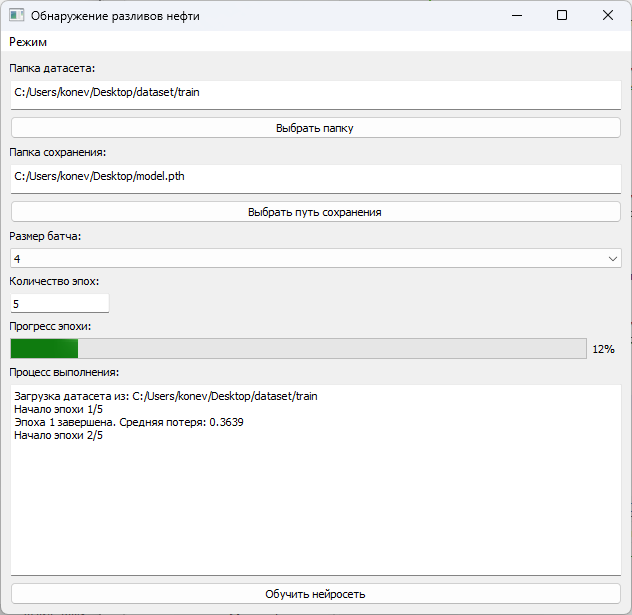
\includegraphics[width=0.7\linewidth]{images/обучение}
	\caption{Процесс обучения нейронной сети}
	\label{fig:training_process}
\end{figure}
\begin{figure}[H]
	\centering
	\includegraphics[width=0.7\linewidth]{"images/обучение результат"}
	\caption{Интерфейс программы после завершения обучения}
	\label{fig:training_result}
\end{figure}
\begin{figure}[H]
	\centering
	\includegraphics[width=0.5\linewidth]{"images/сохраненная модель"}
	\caption{Файл весов модели}
	\label{fig:saved_weights}
\end{figure}

На рисунке~\ref{fig:test_ui_default} изображено окно программы в режиме "<Тестирование">.
\begin{figure}[H]
	\centering
	\includegraphics[width=0.7\linewidth]{"images/тестирование интерфейс"}
	\caption{Окно режима "<Тестирование">}
	\label{fig:test_ui_default}
\end{figure}

На рисунке~\ref{fig:test_image_select} изображено диалоговое окно выбора тестового изображения.
\begin{figure}[H]
	\centering
	\includegraphics[width=0.7\linewidth]{"images/выбор анализируемого изображения"}
	\caption{Диалоговое окно выбора тестового изображения}
	\label{fig:test_image_select}
\end{figure}

На рисунке~\ref{fig:test_model_select} изображено диалоговое окно выбора тестируемых весов.
\begin{figure}[H]
	\centering
	\includegraphics[width=0.7\linewidth]{"images/выбор тестовой модели"}
	\caption{Диалоговое окно выбора тестируемой модели}
	\label{fig:test_model_select}
\end{figure}

На рисунке~\ref{fig:test_results_show} отображены результаты тестирования выбранных весов модели нейронной сети.
\begin{figure}[H]
	\centering
	\includegraphics[width=0.7\linewidth]{"images/результаты теста"}
	\caption{Результаты тестирования}
	\label{fig:test_results_show}
\end{figure}

\subsection{Сборка программной системы}

Программные компоненты представляют собой файлы исходных кодов программной системы.

Для сборки и компиляции программной системы использовалась библиотека Pyinstaller, позволяющая упаковать все необходимые файлы в один исполняемый файл формата .exe. Данный файл может быть запущен без предварительной установки.

Интерпретация исходных кодов на языке Python выполняется встроенным в исполняемый файл интерпретатором языка и не требует отдельной установки интерпретатора и библиотек на целевую систему.

Все программные компоненты собраны в один исполняемый файл, готовый к запуску в среде Windows.